
%
% An example of how to use the unmthesis document class
%

%
% Step 1: Use the unmthesis document class
%
% The class defaults to double spacing
% The [singlespace] option overrides the default doublespacing
% As of November 2020, the final dissertation should be formatted in doublespace
%
\documentclass[singlespace]{../unmthesis}

%
% Step 2: Add whatever packages you need
%
\usepackage{graphicx}
\usepackage{subcaption}
\usepackage{booktabs}
\usepackage{multirow}

%
% Step 3: The bibliography
%
% The unmthesis.cls document class is set up to use biber to generate the bibliography.
% If you want to use something else (e.g., bibtex), then you will have to edit 
% the bibliography part of the .cls file
%
% Note: if you use biber, include the "bibencoding=utf8" line to avoid 
% compilation errors on systems using older versions of biber that do not 
% default to that encoding.
%
\usepackage[backend=biber,
	url=false, 
  bibencoding=utf8,
  doi=true,
  eprint=false,
	%style=apa, % apa style uses name, date format in inline references
	style=ieee,
	uniquename=false,	% so that first names won't show up inline
]{biblatex}
\addbibresource{refs.bib}

%
% Step 4: 
% Information about you, your thesis, and your committee 
%

% title
\title{The Smelloscope: A finglonger for the nose}

% author
\author{Amy Wong}

% degrees already acquired; omit if not applicable
\degreeheld{B.A., Oxnard State University, 1999\\
M.S., Easter Island Polytechnic Institute, 2002}

% month, year this PhD is to be awarded 
\graddate{December}{2020}

% Committee members; the class definition expects four but the .cls file can be easily edited to allow more or less
\cnameone{Hubert Farnsworth}
\caffiliationone{Mars University}
\cnametwo{Hermes Conrad}
\caffiliationtwo{Bureaucrat, Grade 34}
\cnamethree{Phillip J. Fry}
\caffiliationthree{Panucci's Pizza}
\cnamefour{Melllvar}
\caffiliationfour{Planet Omega 3}

%
% Step 5:
% 
% Generate the approval page, the title page, the dedication page, the acknowledgements page, 
% the abstract, the table of contents, etc.
%

% The usual document beginning
\begin{document}

% start the front matter (REQUIRED for formatting)
\frontmatter

% the approval page, listing your committee members etc.
\makeapproval % REQUIRED

% the title page
\maketitle		% REQUIRED

% dedication page
\begin{dedication}	% optional
This work is dedicated to Dr. Hubert Farnsworth, whose magnificent finglonger, had it 
existed in the actual world, would surely have inspired 
me to dream of a world where happiness is perpendicular to wonderment.
\end{dedication}

% acknowledgements page
\begin{acknowledgements} % optional
I acknowldege nothing.
\end{acknowledgements}

% abstract
\begin{abstract} % REQUIRED
\textbf{November 2020: UNM graduate studies says the abstract must be $\leq 150$ words.}
For centuries, mankind has irrationally limited themselves to utilizing only one 
of the five senses in the exploration of the universe: sight. In this 
work, I present the Smelloscope, a device that vastly expands our ability to gain information 
regarding distant objects by leveraging the power of \emph{smell}. 
After describing how the device works, I present a detailed case 
study involving a giant ball of garbage that, without the aid of the Smelloscope, would have 
destroyed the Earth.
\end{abstract}

% long abstract, if you want it
\begin{longabstract}
If you want a longer abstract, it can go here. The unmthesis.cls file can be 
edited if you want the title, your name, etc. to appear on the long abstract 
in the same way it appears with the short abstract.
\end{longabstract}

% make the table of contents
\makecontents % REQUIRED

%
% Step 6: The main part of the dissertation, i.e., all the writing, i.e. the `body of work'
%

% start the body of work (REQUIRED for formatting)
\bodyofwork

%
% For chapters, use the standard \chapter command 
%
% For sections, subsections, etc., use the standard \section, \subsection, etc. commands
%
\chapter{The Five Senses}\label{chapter:01}

The five senses are (1) touch, (2) extrasensory perception, (3) smell, (4) electricity, and (5) the ethereal plane. 
Of these, smell is the least well-understood.

\section{The nose}\label{sec:nose}

While the knees and elbows are well-known olfactory organs, in humans the 
primary instrument of smell is the \emph{nose} or `human horn'~\parencite{baudrillard_simulacra_1994, borges_tlon_nodate}. 
Figure~\ref{fig:nose} illustrates an average horn of the sort one might find on any 
human. 

%
% For figures, use the standard figure environment
%
\begin{figure}[ht]
\centering
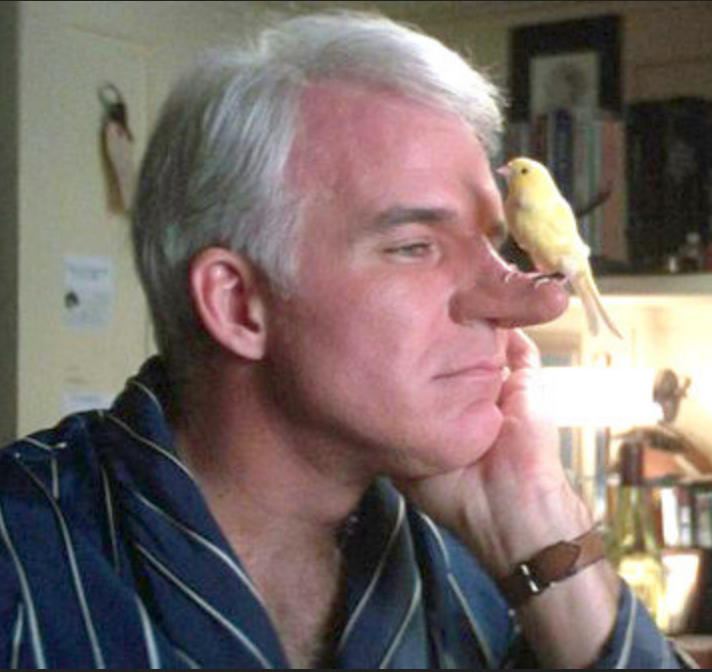
\includegraphics[width=0.45\textwidth]{./figures/human-with-horn}
\caption{A typical human nose.}
\label{fig:nose}
\end{figure}

Amongst some cultures, the human horn is considered an aphrodisiac, and there currently exists a thriving black 
market for noses. Consequently, this valuable resource must be carefully monitored; 
Figure~\ref{fig:poaching} illustrates the unfortunate outcome of a failure to maintain proper vigilance.

\begin{figure}[ht]
\centering

\includegraphics[width=0.45\textwidth]{./figures/human-without-horn}
\caption{The heartbreaking results of nose poaching.}
\label{fig:poaching}
\end{figure}

Table~\ref{tab:lengths} provides a broad overview of nose lengths as they appear in the human population.

%
% For tables, use the standard table environment
%
\begin{table}[ht]
    \centering
    \begin{tabular}{lc}
        \toprule
				Subject & Length (inches)\\
				\midrule
			  Cyrano de Bergerac & 3.1\\
				Adam Driver & 4.6\\
        Pinnochio & 22.3 \\
        Dumbo & 75\\
        \bottomrule
    \end{tabular}
    \caption{Representative human nose lengths.}
    \label{tab:lengths}
\end{table}

\chapter{The Smelloscope}\label{chapter:02}

In this chapter we introduce the Smelloscope, the most revolutionary advance in technology since Betamax brought 
Hollywood into the living room. In section~\ref{sec:smelloscope} we describe how the device works, and in Section~\ref{sec:usage} discuss its proper usage. 

\section{How the Smelloscope works}\label{sec:smelloscope}

Space is permeated with smells. Like light, smell behaves as both a wave (`stink lines'; cf. 
Figure~\ref{fig:stink-lines}) and a particle, depending on how it is observed. 
\begin{figure}[h]
\centering

\includegraphics[width=0.45\textwidth]{./figures/stink-lines}
\caption{Smell in its wave form.}
\label{fig:stink-lines}
\end{figure}

The Smelloscope harvests smell particles as they blast through the universe, concentrating them via 
an olfactory lens, and delivering the results to the observer through a human-Smelloscope nostril 
interface (HSNI). Figure~\ref{fig:smelloscope} shows the original Smelloscope (left), installed at the 
Planet Express delivery service headquarters in New New York, and a more recent, portable version (right).

\begin{figure}[ht]
\centering
\begin{subfigure}[b]{0.4\textwidth}
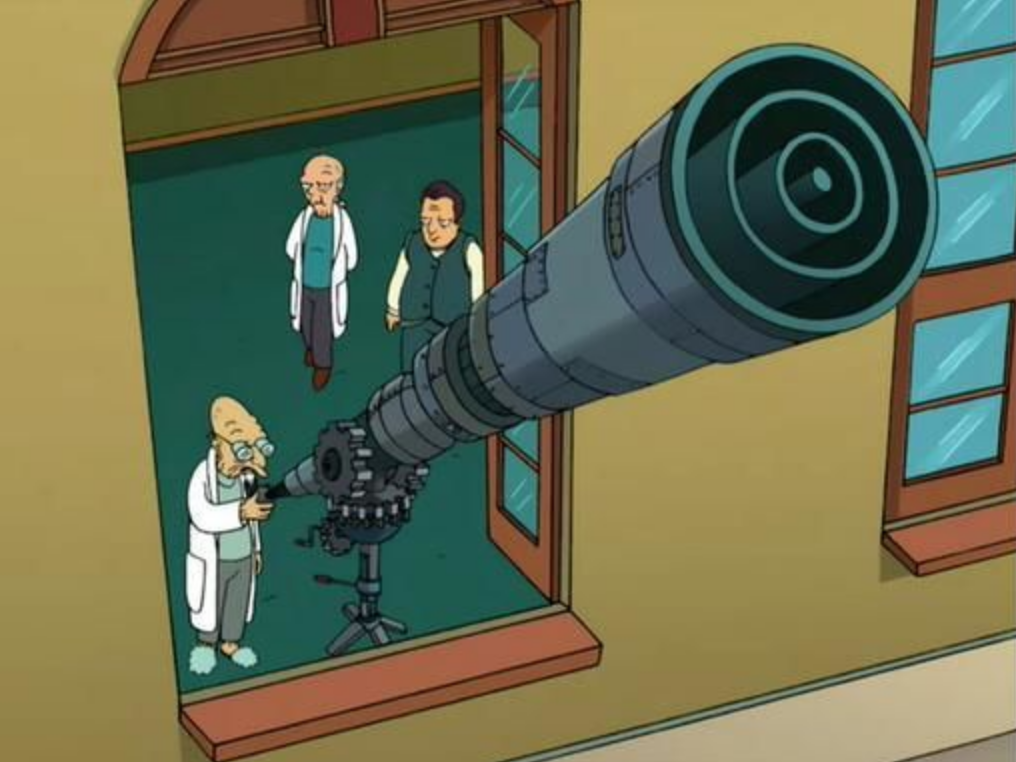
\includegraphics[width=\textwidth]{./figures/smelloscope01}
\end{subfigure}
\hfill
\begin{subfigure}[b]{0.4\textwidth}
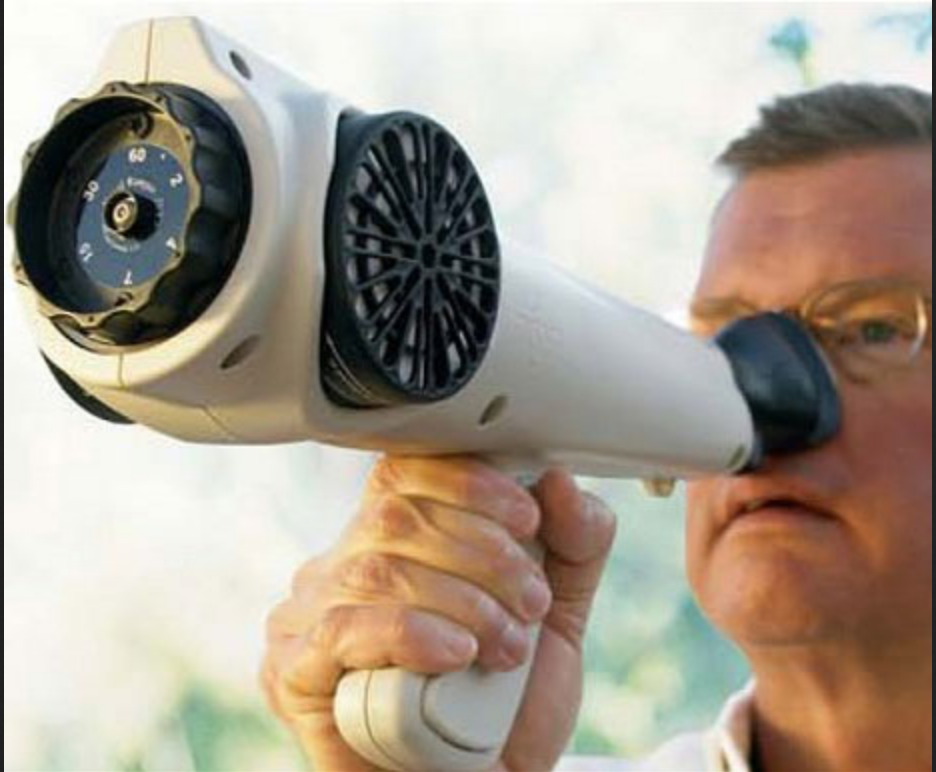
\includegraphics[width=\textwidth]{./figures/smelloscope03}
\end{subfigure}
\caption{The original Smelloscope (left), and a portable version (right)}
\label{fig:smelloscope}
\end{figure}

\section{Proper usage}\label{sec:usage}

Like the colors of the rainbow, smells come in diverse flavors, from sweet to tangy to horse. 
Therefore, great care must be taken when inhaling through the HSNI. Figure~\ref{fig:smelloscope04} 
illustrates the dire consequences that can follow from not following proper Smelloscope procedures.

\begin{figure}[ht]
\centering

\includegraphics[width=0.45\textwidth]{./figures/smelloscope04}
\caption{Gag reflex triggered by incorrect Smelloscope usage.}
\label{fig:smelloscope04}
\end{figure}


%
% Step 7: Appendices
%
% The UNM thesis guidelines impose specific requirements on the formatting for appendices, 
% including a list of appendices and guidelines for how how they are presented in the table of contents.
%
% For this reason, we've defined some special appendix-related commands.
%
% The appendices begin with \appendixstart and end with \appendixend
%
\appendixstart

% Each appendix is introduced with \addappendix{<title of appendix>}
\addappendix{Smelloscope schematics}
This is where the schematics go.

% For reasons explained in the .cls file (basically TOC numbering), you have to use \appsection instead of \section
\appsection{First schematic appendix section}
This is a section of an appendix.


\appsection{Second section}
This is another section of an appendix.


\addappendix{Smelloscope timeline}
A timeline of Smelloscope innovations and milestones would go here if there is one.


\appsection{Still another section}
This is another section of another appendix.

\appendixend


%
% Step 8: wrap things up
%
% Add your references.
\references{}

% end the document
\end{document}
